\subsubsection{Dynamics in scene}
Dynamics in the scene can roughly be divided into three separate scenarios, in this section each of them will tested in a controlled environment with each scenario isolated to show how the signal and the reconstructed image is effected.\\[0.1in]

In the first scenario a object will be placed in an image but for each measurement matrix the location of the object will be moved in a bounded area of the image. This will model as a scene where the background is static but a person is standing in the same spot but moving around.

\begin{figure}[H]
    \centering
\begin{minipage}[t]{0.32\textwidth}
    \includegraphics[width=1\textwidth]{result/dynamic/local/local_whole_time_org.png}
    \subcaption{Original reference image}
    \label{fig:local_1}
\end{minipage}
\begin{minipage}[t]{0.32\textwidth}
    \includegraphics[width = \textwidth]{result/dynamic/local/local_whole_time_ref.png}
    \subcaption{Reconstructed $30\%$ image from reference image without movement}
    \label{fig:local_2}
\end{minipage}
\begin{minipage}[t]{0.32\textwidth}
    \includegraphics[width = \textwidth]{result/dynamic/local/local_whole_time_res_psnr_29_snr_25_sssim_91.png}
    \subcaption{Reconstructed $30\%$ image with local movement}
    \label{fig:local_3}
\end{minipage}
    \caption{Local movement}
    \label{fig:local_dyn}
\end{figure}

The difference between figure~\ref{fig:local_2} and \ref{fig:local_3} is visible with the naked eye, not only does the object moving around get blurry and noisy but the whole image globally. In table~\ref{tab:local_dyn}...

\begin{table}[H]
    \centering
  \begin{tabular}{ | l | l | l |}
    \hline
    Peak SNR & SNR & SSIM \\ \hline
    29 & 25 & 91 \\ 
    \hline
  \end{tabular}
      \caption{Effects comparing non perturbed reconstructed image against reconstructed image with local movement}
    \label{tab:local_dyn}
\end{table}

Commenting the result from the table... In figure~\ref{fig:local_sig} the effects of the movement is shown plotted against the non perturbed signal.\\[0.1in]

\begin{figure}[H]
    \centering
\begin{minipage}[t]{0.495\textwidth}
    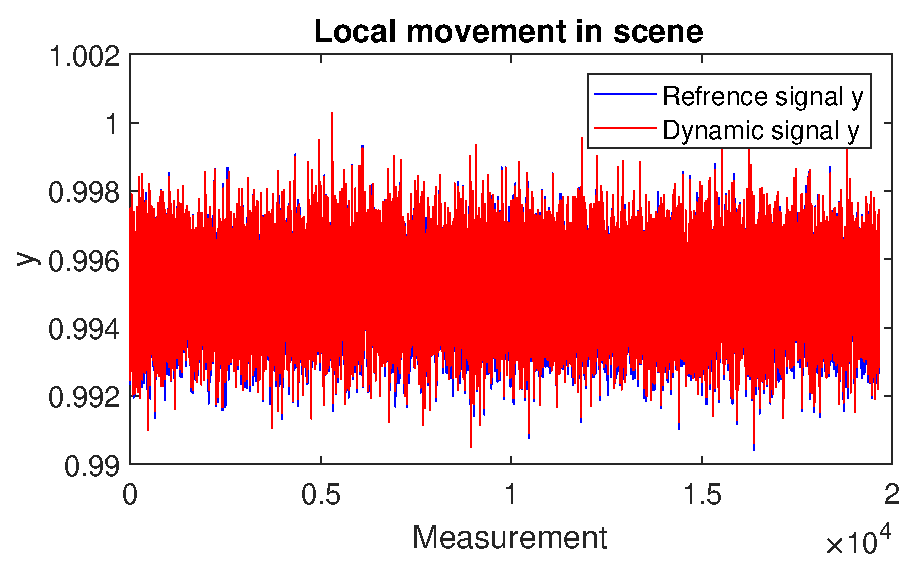
\includegraphics[width=1\textwidth]{result/dynamic/local/local_whole_time.eps}
    \subcaption{Signal.}
    \label{fig:local_sig_1}
\end{minipage}
\begin{minipage}[t]{0.495\textwidth}
    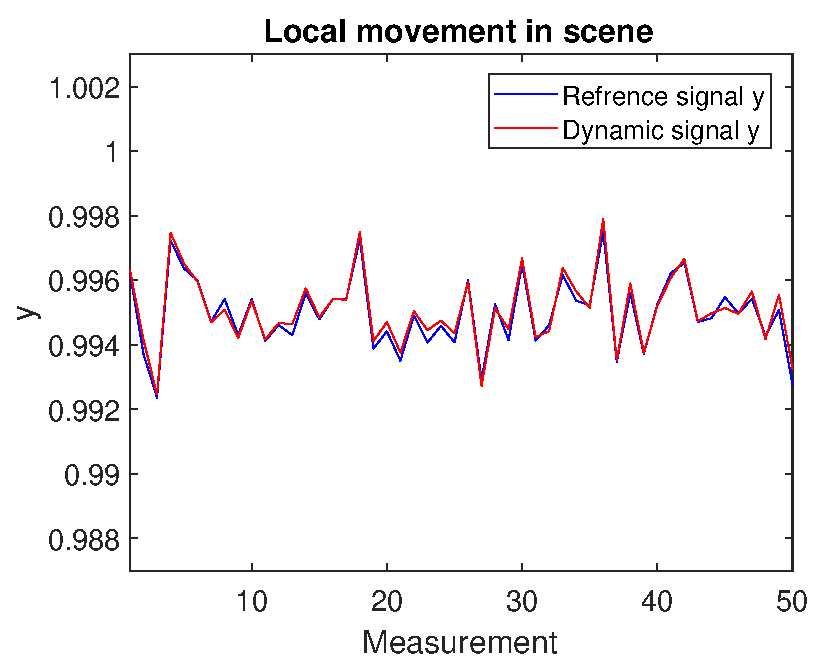
\includegraphics[width = \textwidth]{result/dynamic/local/local_whole_time_win.eps}
    \subcaption{Zoomed in view of the signal.}
    \label{fig:local_sig_2}
\end{minipage}
    \caption{Local movement, acquired signal}
    \label{fig:local_sig}
\end{figure}


As seen in figure~\ref{fig:local_sig_1} there is no obvious difference between the non perturbed reference signal and the distorted signal. In figure~\ref{fig:local_2} where some of the samples is displayed no large difference can be seen ether, the conclusion of this test implies that local movement in a scene will cause noise in the image globally and especially locally where the movement occurred. It also implies that local movement is very hard to detect on the signal even if a reference signal is available.\\[0.1in] 

%%%%%%%%%% Second scenario %%%%%%%%%%%%%%%%

The second scenario is an object is passing through, moves out or moves to an other place in the scene far from the original place. In other words, large global movement in the scene. The problem is modeled with a static background then as the simulated measurement is acquired the same object as in the first experiment will cross the scene, like a car,human or animal might do when using the SPC. The object will cross the scene in 1000 measurements of approximately 19000, corresponding to approximately $0.7$ seconds when capturing with the SPC in its current setup.



\begin{figure}[H]
    \centering
\begin{minipage}[t]{0.32\textwidth}
    \includegraphics[width=1\textwidth]{result/dynamic/fly/flyby_1sec_org.png}
    \subcaption{Original reference image}
    \label{fig:fly_1}
\end{minipage}
\begin{minipage}[t]{0.32\textwidth}
    \includegraphics[width = \textwidth]{result/dynamic/fly/flyby_1sec_ref.png}
    \subcaption{Reconstructed $30\%$ image from reference image without movement}
    \label{fig:fly_2}
\end{minipage}
\begin{minipage}[t]{0.32\textwidth}
    \includegraphics[width = \textwidth]{result/dynamic/fly/flyby_1sec_res_psnr_23_snr_18_sssim_58.png}
    \subcaption{Reconstructed $30\%$ image with object passing trough}
    \label{fig:fly_3}
\end{minipage}
    \caption{Object passing trough scene.}
    \label{fig:fly_dyn}
\end{figure}

The difference between figure~\ref{fig:fly_2} and \ref{fig:fly_3} is visible with the naked eye, A global noise arises in the image and the object cant be seen. In table~\ref{tab:fly_dyn}...


\begin{table}[H]
    \centering
  \begin{tabular}{ | l | l | l |}
    \hline
    Peak SNR & SNR & SSIM \\ \hline
    23 & 18 & 58 \\ 
    \hline
  \end{tabular}
      \caption{Effects comparing non perturbed reconstructed image against reconstructed image with local movement}
    \label{tab:fly_dyn}
\end{table}


Commenting the result from the table... In figure~\ref{fig:fly_sig} the effects of the movement is shown plotted against the non perturbed signal.\\[0.1in]


\begin{figure}[H]
    \centering
\begin{minipage}[t]{0.495\textwidth}
    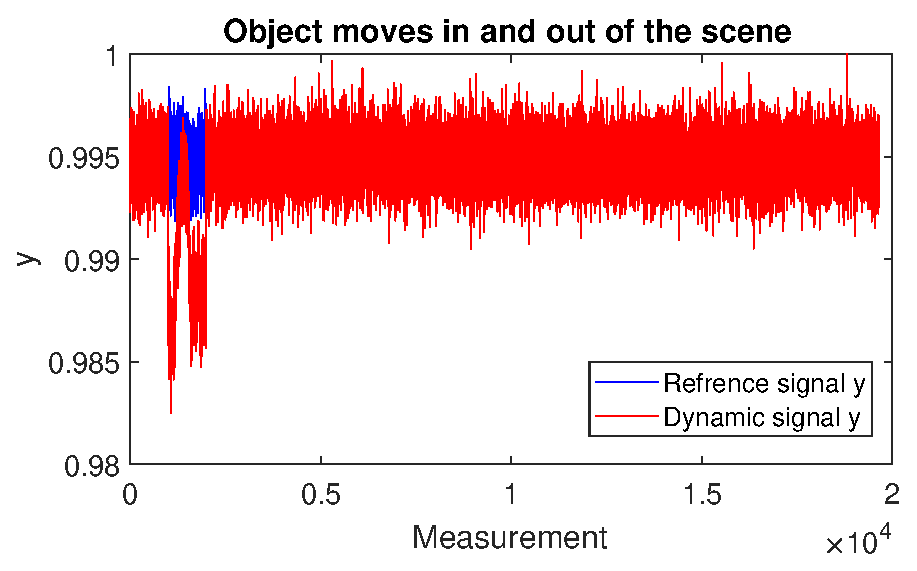
\includegraphics[width=1\textwidth]{result/dynamic/fly/flyby_sig.eps}
    \subcaption{Signal.}
    \label{fig:fly_sig_1}
\end{minipage}
\begin{minipage}[t]{0.495\textwidth}
    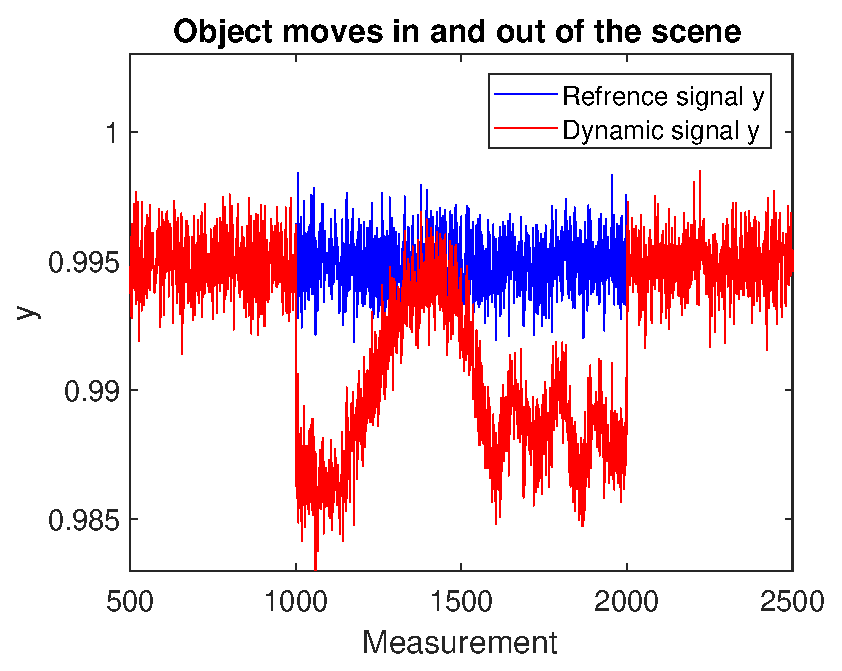
\includegraphics[width = \textwidth]{result/dynamic/fly/flyby_plot_win.eps}
    \subcaption{Zoomed in view of the signal.}
    \label{fig:fly_sig_2}
\end{minipage}
    \caption{Global movement, acquired signal}
    \label{fig:fly_sig}
\end{figure}

\begin{itemize}
    \item Large changes in the scene can be detected
    \item Remove the identified measurements to get a good signal 
\end{itemize}

%%%%%%%%%%%% Third %%%%%%%%%%%%%%%

The third scenario i luminance change in the scene caused by clouds occludes the sun or the light intensity from the lights is not constant. This scenario is modeled by adding or subtracting the global intensity in the image over the measurements. 

\begin{figure}[H]
    \centering
\begin{minipage}[t]{0.245\textwidth}
    \includegraphics[width=1\textwidth]{result/dynamic/lum/intense_change_org.png}
    \subcaption{Original reference image}
    \label{fig:lum_1}
\end{minipage}
\begin{minipage}[t]{0.245\textwidth}
    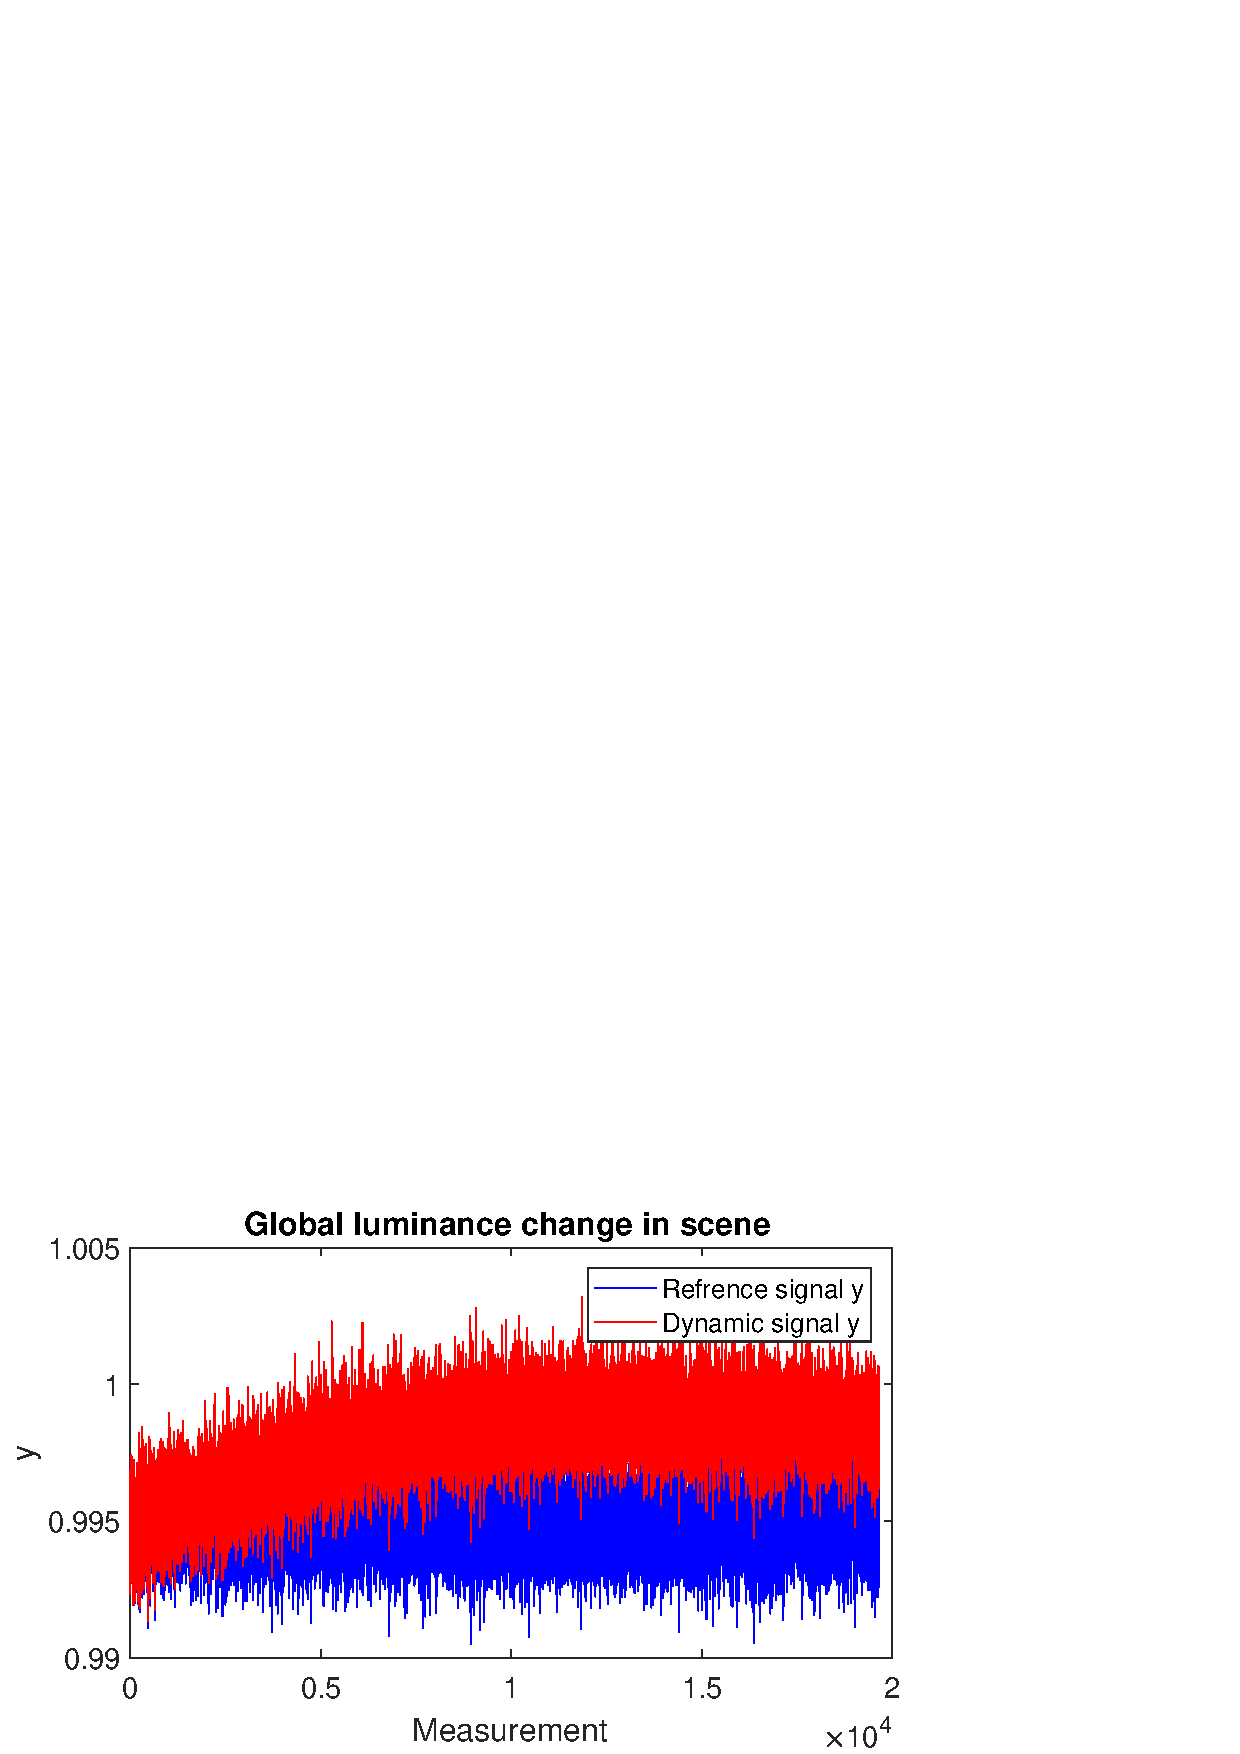
\includegraphics[width = \textwidth]{result/dynamic/lum/intense_change.png}
    \subcaption{Reconstructed $30\%$ image from reference image without movement}
    \label{fig:lum_2}
\end{minipage}
\begin{minipage}[t]{0.245\textwidth}
    \includegraphics[width = \textwidth]{result/dynamic/lum/intense_change_psnr_19_snr_14_sssim_38.png}
    \subcaption{Reconstructed $30\%$ image with global luminance change}
    \label{fig:lum_3}
\end{minipage}
\begin{minipage}[t]{0.245\textwidth}
    \includegraphics[width = \textwidth]{result/dynamic/lum/intense_change_movemean_psnr_33_snr_29_sssim_93.png}
    \subcaption{Reconstructed $30\%$ image with mean subtraction}
    \label{fig:lum_4}
\end{minipage}
    \caption{Global luminance change in scene.}
    \label{fig:lum_dyn}
\end{figure}


The difference between figure~\ref{fig:lum_2} and \ref{fig:lum_3} is visible with the naked eye, A global noise arises in the image, but as seen in figure~\ref{fig:lum_4} the effect can be suppressed explained under figure~\ref{fig:lum_sig}. In table~\ref{tab:fly_dyn}...


\begin{table}[H]
    \centering
  \begin{tabular}{ | l | l | l | l |}
    \hline
     & Peak SNR & SNR & SSIM \\ \hline
    Perturbed signal & 19 & 14 & 38 \\ \hline
    Mean subtracted signal & 33 & 29 & 93 \\
    \hline
  \end{tabular}
      \caption{Effects comparing non perturbed reconstructed image against reconstructed image with global luminance change}
    \label{tab:lum_dyn}
\end{table}


Commenting the result from the table... In figure~\ref{fig:lum_sig} the effects of global luminance is shown plotted against the non perturbed signal.\\[0.1in]


\begin{figure}[H]
    \centering
\begin{minipage}[t]{0.495\textwidth}
    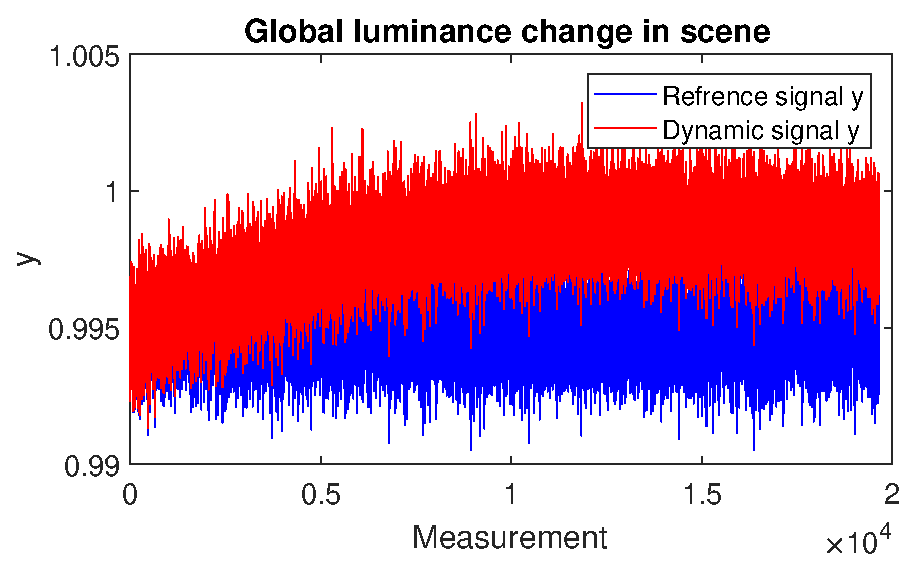
\includegraphics[width=1\textwidth]{result/dynamic/lum/intense_change.eps}
    \subcaption{Signal.}
    \label{fig:lum_sig_1}
\end{minipage}
\begin{minipage}[t]{0.495\textwidth}
    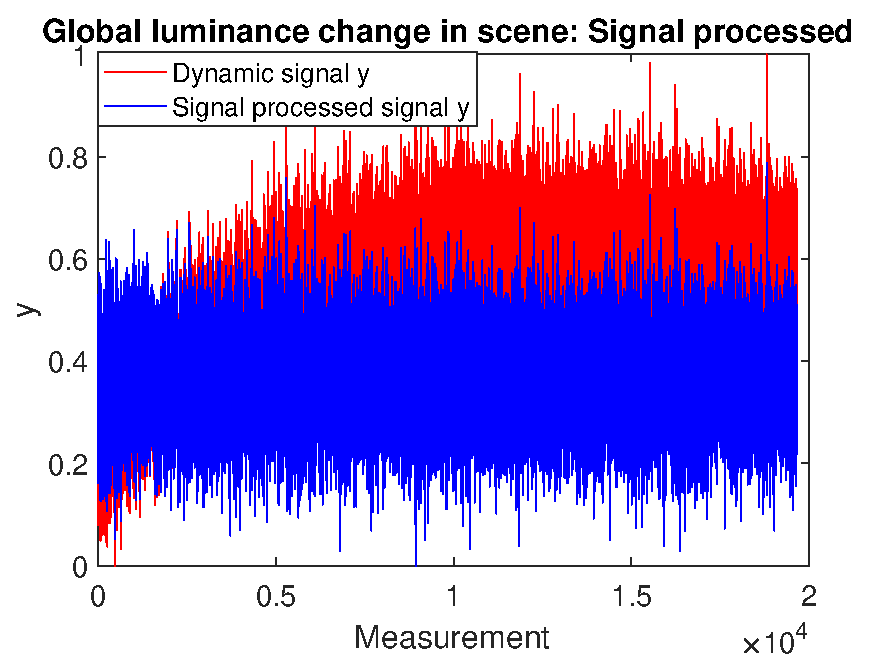
\includegraphics[width = \textwidth]{result/dynamic/lum/intense_change_sp.eps}
    \subcaption{Zoomed in view of the signal.}
    \label{fig:lum_sig_2}
\end{minipage}
\begin{minipage}[t]{0.495\textwidth}
    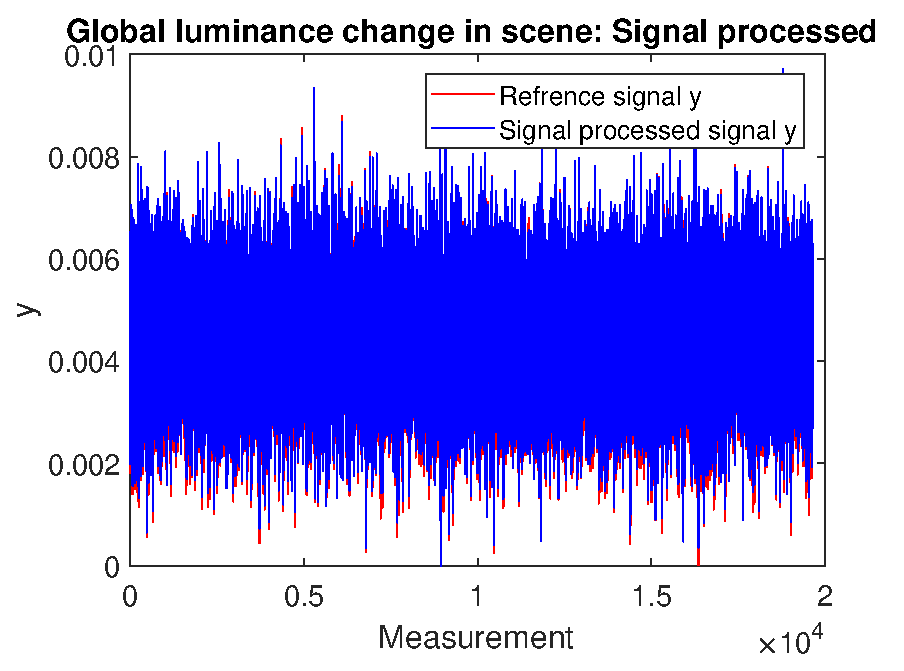
\includegraphics[width=1\textwidth]{result/dynamic/lum/intense_change_sp_ref.eps}
    \subcaption{Signal.}
    \label{fig:lum_sig_3}
\end{minipage}
\begin{minipage}[t]{0.495\textwidth}
    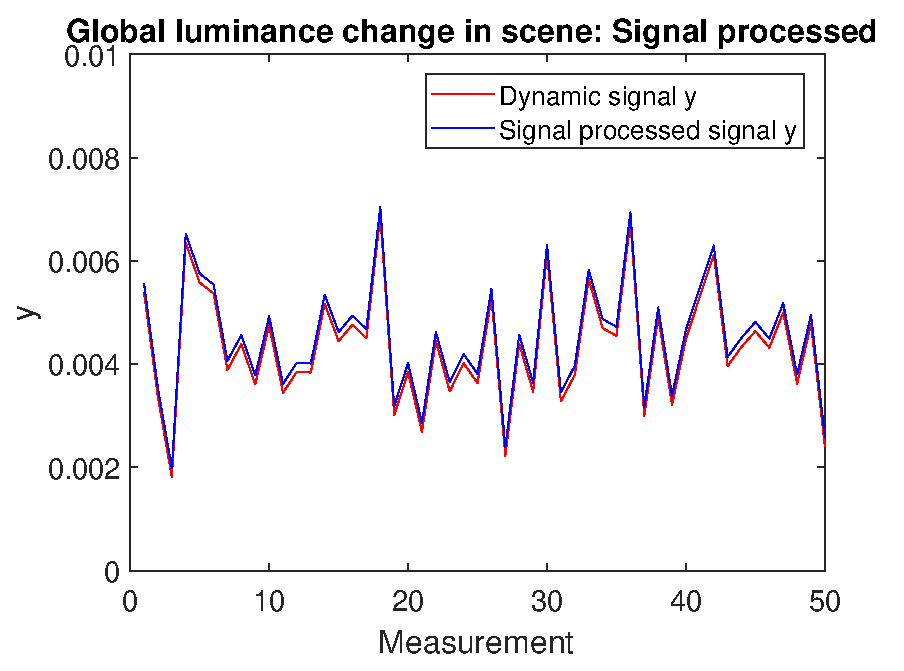
\includegraphics[width = \textwidth]{result/dynamic/lum/intense_change_sp_ref_win.eps}
    \subcaption{Zoomed in view of the signal.}
    \label{fig:lum_sig_4}
\end{minipage}
    \caption{Global movement, acquired signal}
    \label{fig:lum_sig}
\end{figure}

\begin{itemize}
    \item Dynamic signal v. Reference signal
    \item Dynamic signal v. Mean subtracted signal
    \item Reference signal v. Mean subtracted signal
    \item Comment on the window, pretty good.
    \item Can be detected with the knowledge that the signal should be stationary. Signal process the signal to look like a stationary signal.
\end{itemize}